\documentclass[11pt]{article}

% ── Packages ────────────────────────────────────────────────
\usepackage[margin=1in]{geometry}
\usepackage{amsmath, amssymb, amsthm}
\usepackage{booktabs}
\usepackage{graphicx}
\usepackage{hyperref}
\usepackage{natbib}
\usepackage{setspace}
\usepackage{microtype}
\usepackage{enumitem}
\usepackage{caption}
\usepackage{subcaption}
\usepackage{xcolor}
\usepackage{float}
% code packages
\usepackage{listings}
\usepackage{inconsolata}
\lstset{basicstyle=\ttfamily\footnotesize,breaklines=true}
\usepackage{csvsimple}
\usepackage{booktabs}

% ── Hyperref setup ──────────────────────────────────────────
\hypersetup{
    colorlinks = true,
    linkcolor  = black,
    citecolor  = black,
    urlcolor   = blue
}

% ── Theorem environments ────────────────────────────────────
\newtheorem{theorem}{Theorem}
\newtheorem{proposition}{Proposition}
\newtheorem{lemma}{Lemma}
\newtheorem{corollary}{Corollary}
\theoremstyle{definition}
\newtheorem{definition}{Definition}
\newtheorem{assumption}{Assumption}
\theoremstyle{remark}
\newtheorem{remark}{Remark}

% ── Spacing ─────────────────────────────────────────────────
\onehalfspacing

% ── Title block ─────────────────────────────────────────────
\title{Love of Variety: July 27th Update}
\author{Tate Mason}
\date{\today}

% ============================================================
\begin{document}
\maketitle
\thispagestyle{empty}

\section{Overview}

This document serves to provide all relevant statistics and graphics garnered thus far in the Love of Variety research for my second year paper. My hope is that we are moving towards estimation with this smaller subset of data before expansion to other categories of products. I will be providing summary stats for the sample, statistics for switching behavior, graphics for variety seeking behavior, and then some graphics and statistics for the specific ways people switch.

My sample is of single person households in all markets. I filter to households which make at least two shopping trips. I created flavor bins at varying levels. First, specific buckets: 13 unique flavor buckets for popular flavors. Second, binary buckets: plain or flavored yogurt. Finally, the preferred three-bucket specification: berry, plain, other. This is preferred due to simplifying the dimensions of characteristics while also keeping variation in types of flavors. 

\section{Summary Statistics}

Below, I list a table of summary statistics in table \ref{tab:desc_stats}. The sample consists of 15,440 households which are seen for 16 trips on average. Each household purchases 2 yogurt cups per trip, on average. About 41\% of the sample take the outside option any given trip. Brand choice is mostly static, with 75\% of households buying the same brand from trip to trip. Flavor, however, is repeated 42\% of trips. This shows that households choose to switch their flavor more than half of the time, on average. Households who are plain type buy plain yogurt more than eight consecutive periods, double the flavored types. Finally, 99\% of households return to a chosen flavor after switching.

\section{Figures}


From the heatmap, we see that all three flavors are relatively close in terms of how long spells of switchig are. These spells range between 2.1 and 2.8 trips, on average. Thus, we see similar variety seeking behaviors when households do switch.

Next, it is worth looking at the granular breakdown of variety when each major flavor has is own bin. When looking at figure \ref{fig:heatmap_granular}, we can see that plain (the final column), has much longer spells on average than the other flavors. For instance, when switching from banana to plain, the household will stay with plain for almost 6 periods. 

When looking at figure \ref{fig:repeat_bar_granular}, we see that plain households will buy plain yogurt 80\% of the time while strawberry, column 10, is 50\%. This further lends itself to plain households being stuck on plain while flavored households are more flexible or variety seeking.

Back to the three-flavor specification, I ran some analysis to tally up how many people are different kinds of switchers (1 bucket, 2 buckets, all buckets). The majority of households are only buying one flavor. This makes sense as plain is the most popular flavor. Close behind is the count of households buying two flavors. Finally, comparatively few households will buy from all three buckets. See figure \ref{fig:bucket_count} below. Table \ref{tab:combo_counts} shows that a majority of the households which do pick two flavors are choosing flavored combinations. This is again reinforcement of the idea that plain households are less prone to switching, making up a third of this sample. 

I started by estimating a simple OLS model. The dependent variable is the probability of switching regressed on age, income, and switching in the previous period. This shows a about a 55\% switching probability, increased by 7\% if switched in the previous period. The structural model is not where I want it. \ref{tab:structural_est} is my first run. I need to go through and tinker with starting values, the moments used, etc. Price should not be zero. That is an obvious error. GACRC is down until Thursday, so I will diagnose in the coming days. I also think some serious consideration needs to be put into disentangling $\beta$ and $\gamma$.


\section{Concluding and Next Steps}

From here, I am beginning structural estimation. Need to decide optimal moments for identifying $\gamma$ which may mean I need to add more structure to the utility function. I also think I need to make some firm decisions on the timing of the model. Things are at the shopping trip level, the purchase date level, or the week level after merging in retail data. Currently I am waffling between trip and purchase date.

\begin{table}[htbp]
    \centering
    \caption{Descriptive Statistics}
    \label{tab:desc_stats}
    \begin{tabular}{lc}
        \toprule
        Statistic & Value \\
        \midrule
        \# Households               & 15668 \\
        Mean \# Times Observed      & 59.01 \\
        Yogurt Purchases            & 3.35 \\
        Mean Income                 & \$16,277 \\
        Median Income               & \$16,000 \\
        \% White                    & 81\% \\
        \% Black                    & 13\% \\
        \% Hispanic                 & 4\% \\
        \% Asian                    & 2\% \\
        \% Taking Outside Option          & 0.49 \\
        Mean Repeat Purchase Rate (Brand)   & 75\% \\
        Mean Repeat Purchase Rate (Flavor)  & 42\% \\
        W/in HH Brand Concentration & 55\% \\
        W/in HH Flavor Concentration& 41\% \\
        Mean Consecutive Buys per HH (Other) & 3.4  \\
        Mean Consecutive Buys per HH (Berry) & 2.5 \\
        Mean Consecutive Buys per HH (Plain) & 6.7 \\
        \% Ever Switched & 35\% \\
        \bottomrule
    \end{tabular}
\end{table}

\begin{figure}[htbp]
  \centering
  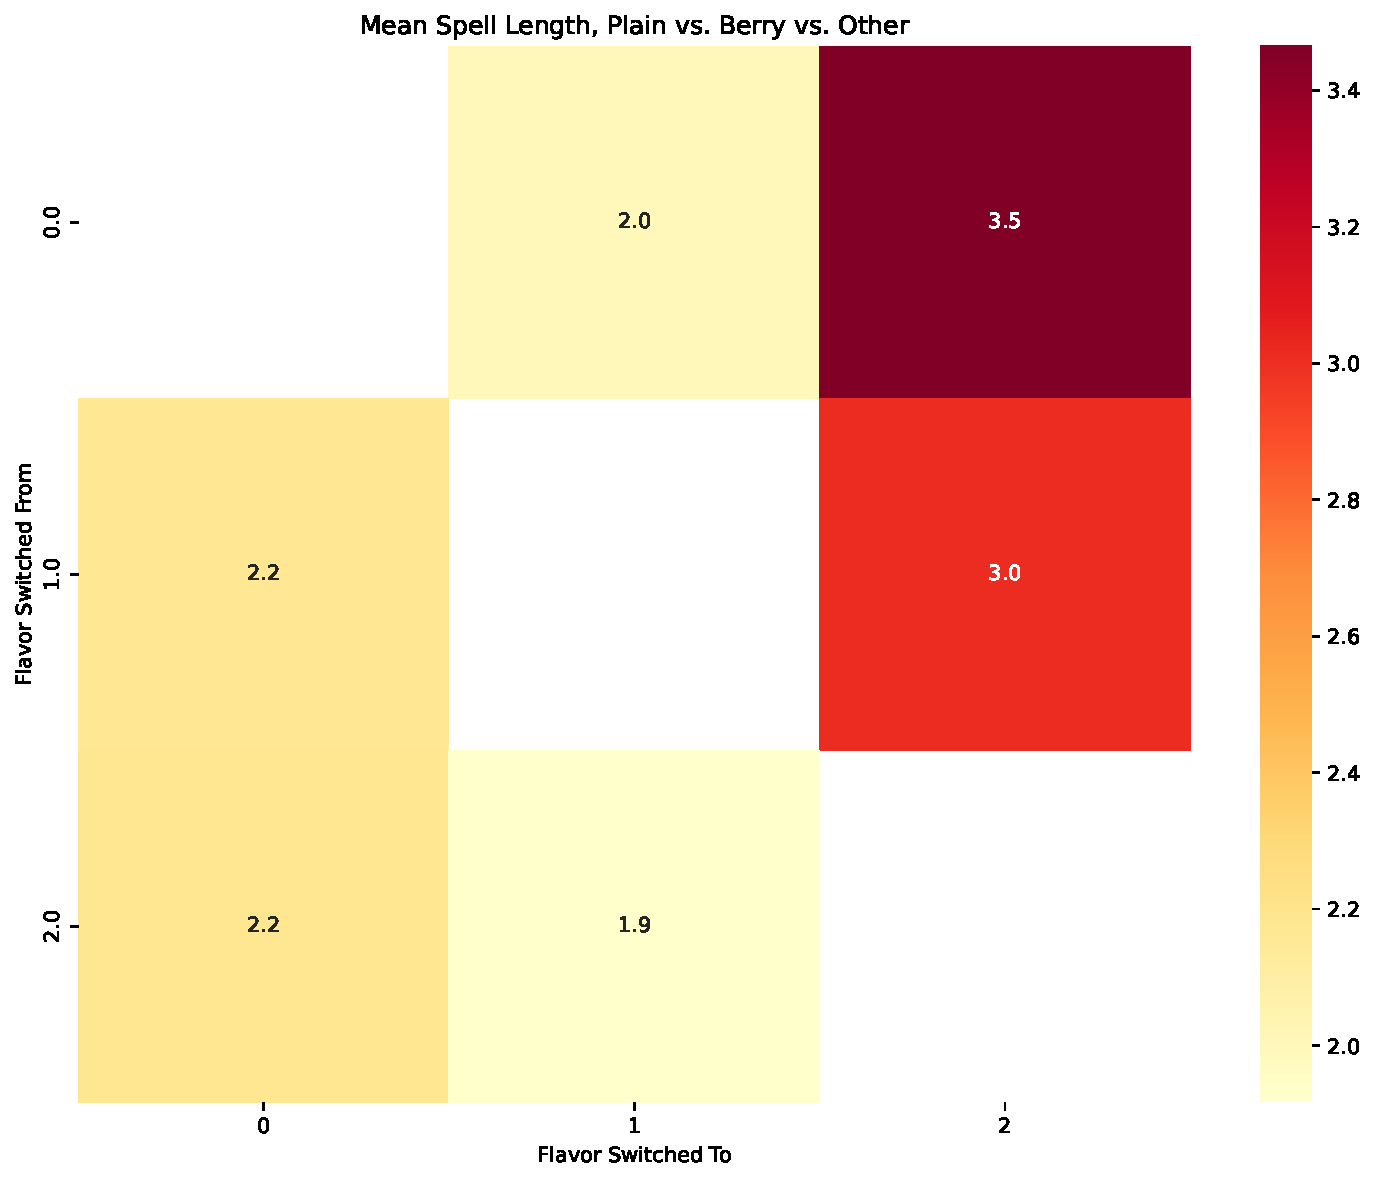
\includegraphics[width=\textwidth]{../../Output/Plots/3flav_heatmap.pdf}
  \caption{}
  \label{fig:heatmap}
\end{figure}

\begin{figure}[htbp]
  \centering
  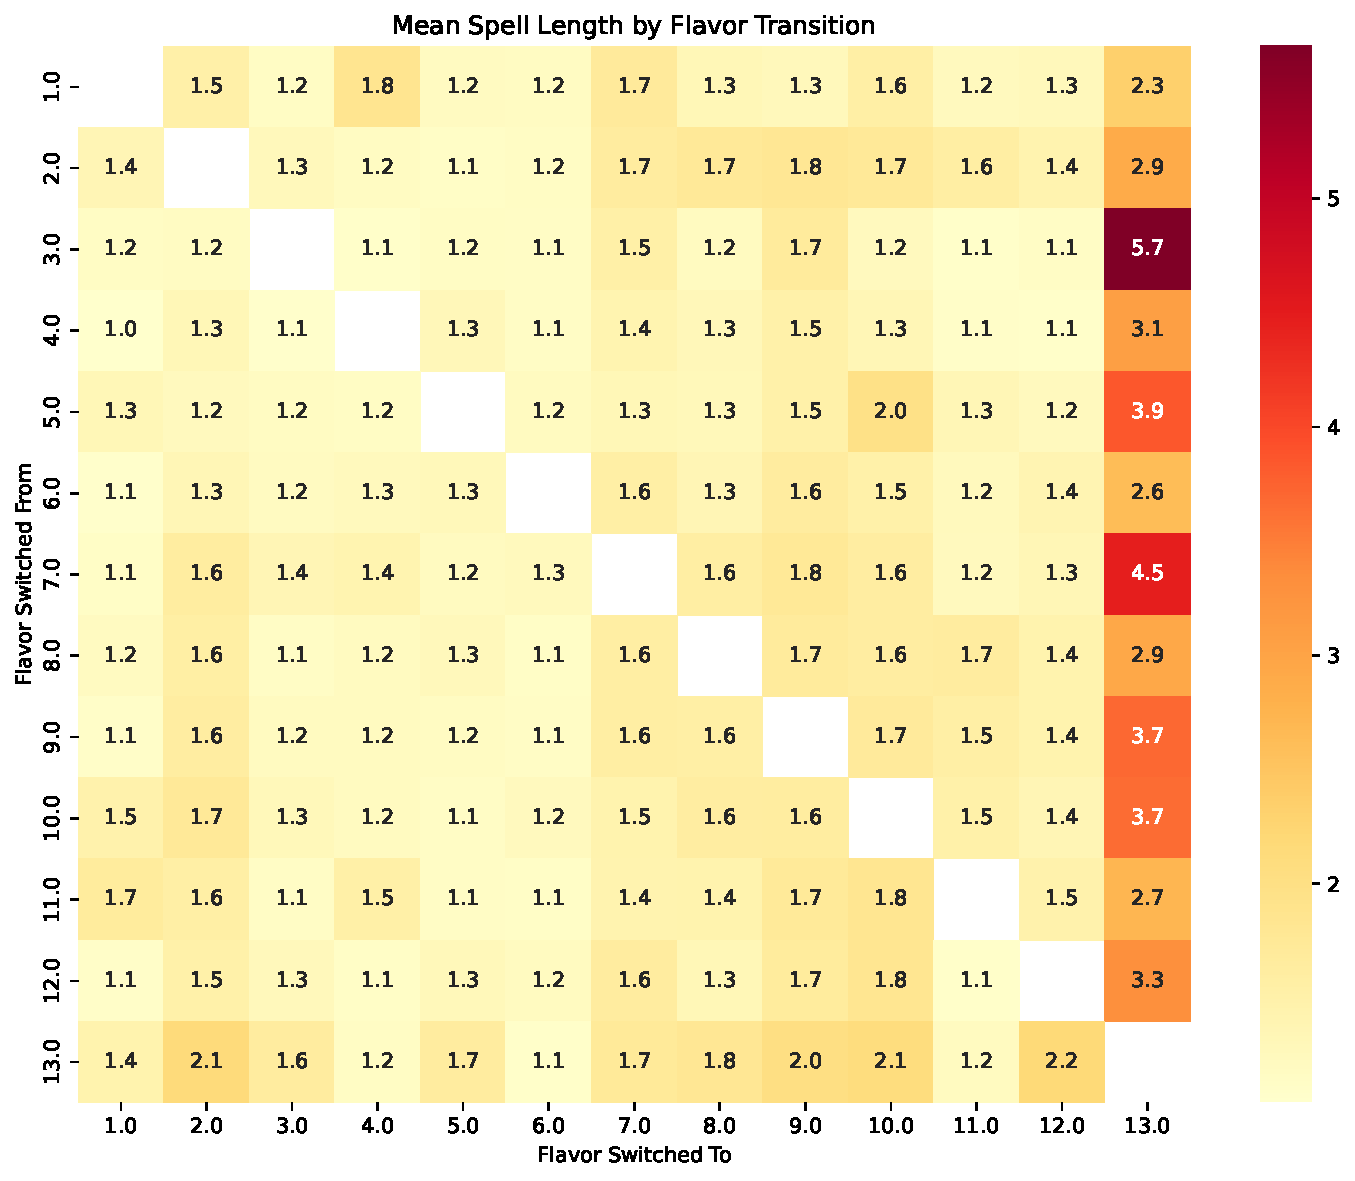
\includegraphics[width=\textwidth]{../../Output/Plots/run_length_heatmap.pdf}
  \caption{}
  \label{fig:heatmap_granular}
\end{figure}

\begin{figure}[htbp]
  \centering
  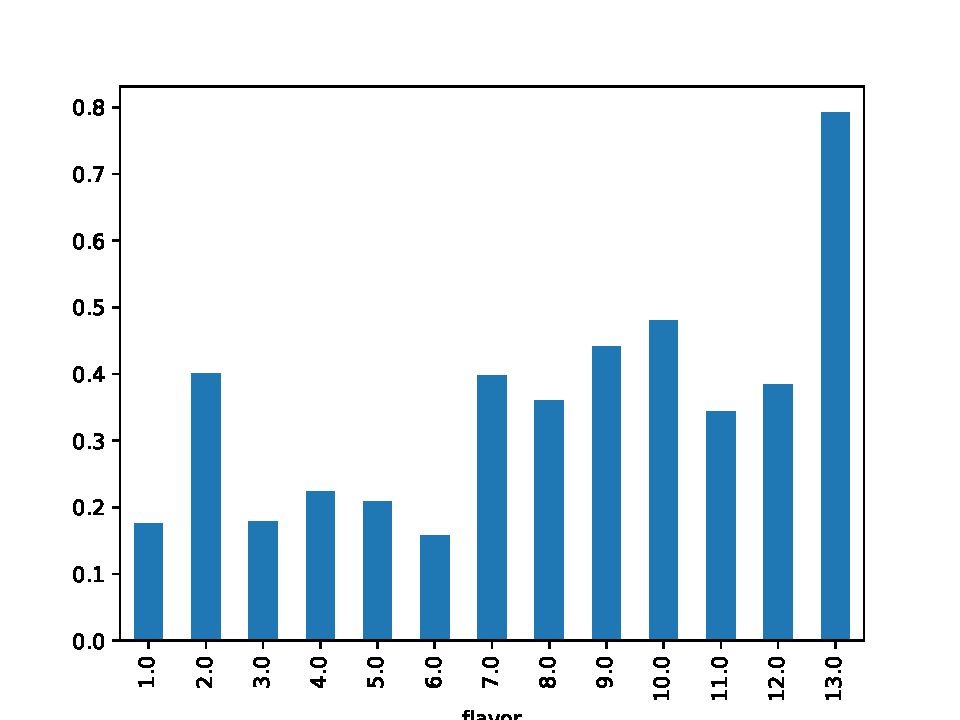
\includegraphics[width=\textwidth]{../../Output/Plots/repeat_flavor_bar.pdf}
  \caption{}
  \label{fig:repeat_bar_granular}
\end{figure}

\begin{figure}[htbp]
	\centering
	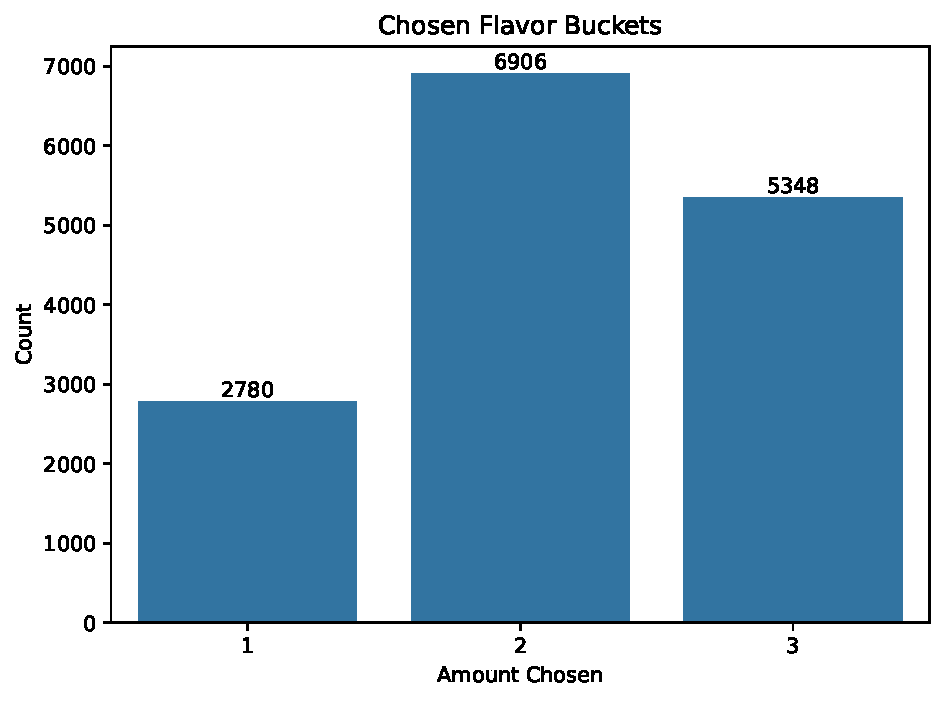
\includegraphics[width=\textwidth]{../../Output/Plots/flavor_pair_comps.pdf}
  \caption{}
	\label{fig:bucket_count}
\end{figure}

\begin{table}[htbp]
	\centering
	\caption{Flavor Combination Counts}
	\label{tab:combo_counts}
	\begin{tabular}{lcc}
		\toprule
		Combination & Count & Percent of Group \\
		\midrule
		Other and Berry & 2659 & 66\% \\
		Other and Plain & 891  & 22\% \\
		Berry and Plain & 478  & 12\% \\
		\bottomrule
	\end{tabular}
\end{table}

\begin{table}[htbp]
  \centering
  \caption{Mean Trips on Flavor Before Switching}
  \label{tab:run_length}
  \begin{tabular}{llc}
      \toprule
      From & To & Mean Trips \\
      \midrule
      Other & Berry & 2.00 \\
      Other & Plain & 3.46 \\
      Berry & Other & 2.17 \\
      Berry & Plain & 3.01 \\
      Plain & Other & 2.18 \\
      Plain & Berry & 1.92 \\
      \bottomrule
  \end{tabular}
\end{table}	

\begin{table}[htbp]
    \centering
    \caption{Flavor Switch Counts (Trip x HH level)}
    \label{tab:switch_matrix}
    \begin{tabular}{lccc}
        \toprule
         & \multicolumn{3}{c}{To} \\
        \cmidrule(lr){2-4}
        From & Other & Berry & Plain \\
        \midrule
        Other & --      & 10{,}673 & 27{,}349 \\
        Berry & 10{,}638 & --      & 9{,}120  \\
        Plain & 27{,}385 & 9{,}246  & --      \\
        \bottomrule
    \end{tabular}
\end{table}

\begin{table}[htbp]
    \centering
    \caption{OLS Regression: Determinants of Flavor Switching}
    \label{tab:ols_switch}
    \begin{tabular}{lc}
        \toprule
         & Switched \\
        \midrule
        \quad Constant & 0.4472$^{***}$ \\
                        & (0.005) \\
        \quad Household Income & 0.0002 \\
                                & (0.000) \\
        \quad Total Price Paid & 0.0094$^{***}$ \\
                                & (0.000) \\
        \quad Male Head Age & $-$0.0009 \\
                             & (0.001) \\
        \quad Female Head Age & $-$0.0009 \\
                               & (0.001) \\
        \quad Switched$_{t-1}$ & 0.0718$^{***}$ \\
                                & (0.002) \\
        \midrule
        Observations & 313{,}475 \\
        $R^2$ & 0.008 \\
        Adjusted $R^2$ & 0.008 \\
        F-statistic & 518.2 \\
        \bottomrule
        \multicolumn{2}{l}{\footnotesize $^{*}p<0.10$, $^{**}p<0.05$, $^{***}p<0.01$} \\
    \end{tabular}
\end{table}

\begin{table}[htbp]
    \centering
    \caption{Structural Model Estimates}
    \label{tab:structural_est}
    \begin{tabular}{lc}
        \toprule
        Parameter & Estimate \\
        \midrule
        $\beta$ (quality utility)        & 1.4152 \\
        $\gamma$ (love of variety)       & 0.8704 \\
        $\alpha$ (price sensitivity)     & 0.0000 \\
        $\lambda$ (habit smoothing)      & 0.6409 \\
        \midrule
        Log-Likelihood & $-$37{,}847.54 \\
        Converged & Yes \\
        \bottomrule
    \end{tabular}
\end{table}


\end{document}


